\documentclass[border=6pt]{standalone}
\usepackage[T1]{fontenc}
\usepackage[utf8]{inputenc}
\usepackage[scaled=0.98]{helvet}
\renewcommand{\familydefault}{\sfdefault}
\usepackage{amsmath}
\usepackage{graphicx}
\graphicspath{{../../../../../../exercises_lecturenotes/lecture_notes/kurs100_lektionsnoter/}}
\usepackage{tikz}
\usepackage{pgfplots}
\pgfplotsset{compat=1.18}
\usetikzlibrary{arrows.meta, decorations.pathreplacing, calc, positioning, fit, backgrounds, shapes.geometric}
\usepgfplotslibrary{groupplots,fillbetween}
\definecolor{scanpink}{HTML}{E5006D}
\definecolor{scanteal}{HTML}{00A6A6}
\definecolor{scannavy}{HTML}{243746}
\definecolor{scanlightgray}{HTML}{F1F2F3}
\begin{document}
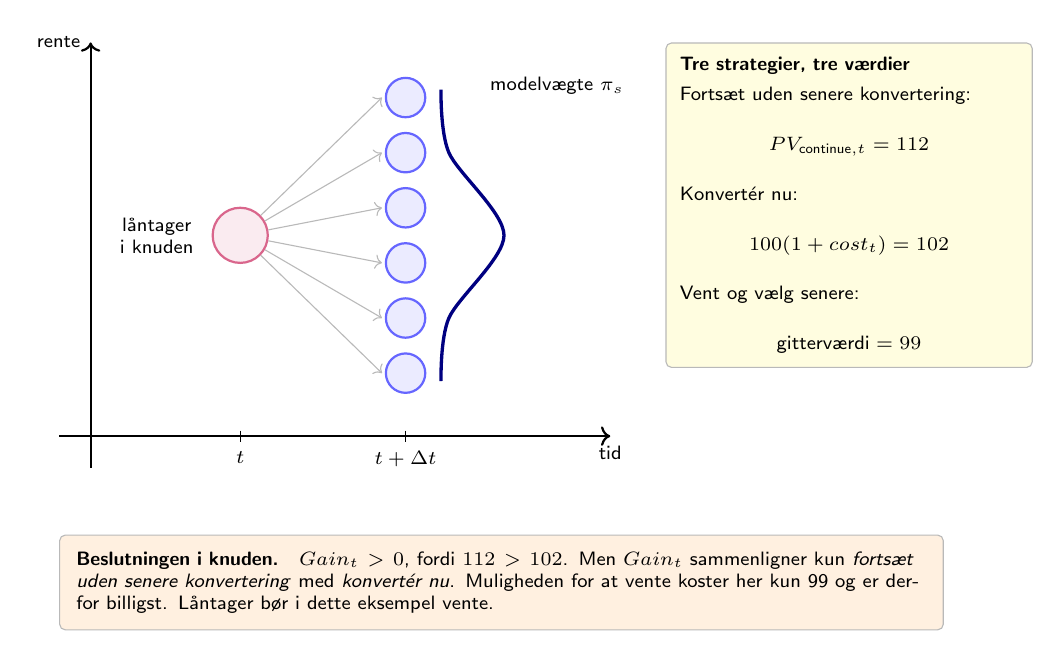
\begin{tikzpicture}[
    font=\scriptsize,
    now/.style={
        circle,
        draw=purple!60,
        thick,
        fill=purple!8,
        minimum size=7mm,
        inner sep=0.5pt
    },
    fut/.style={
        circle,
        draw=blue!60,
        thick,
        fill=blue!8,
        minimum size=5mm,
        inner sep=0.5pt
    },
    warr/.style={
        ->,
        thin,
        gray!55
    },
    note/.style={
        draw=gray!55,
        rounded corners=2pt,
        align=left,
        text width=43mm,
        inner sep=5pt
    },
    widenote/.style={
        draw=gray!55,
        rounded corners=2pt,
        align=left,
        inner sep=6pt
    }
]

% Akser
\draw[->, thick]
    (-0.4,0) -- (6.6,0)
    node[below] {tid};

\draw[->, thick]
    (0,-0.4) -- (0,5.0)
    node[left] {rente};

% Låntagerens aktuelle knude
\node[now] (v) at (1.9,2.55) {};

\node[
    left=3pt of v,
    align=center
] {låntager\\i knuden};

% Mulige tilstande næste termin
\foreach \y in {0.8,1.5,2.2,2.9,3.6,4.3} {
    \node[fut] at (4,\y) {};
    \draw[warr] (v) -- (3.7,\y);
}

% Modelvægtenes illustrative profil
\draw[
    very thick,
    blue!50!black
]
plot[smooth] coordinates {
    (4.45,0.7)
    (4.55,1.5)
    (5.25,2.55)
    (4.55,3.6)
    (4.45,4.4)
};

\node[anchor=west] at (4.95,4.45)
    {modelvægte \(\pi_s\)};

% Tidsmarkeringer
\draw
    (1.9,0.07) -- (1.9,-0.07)
    node[below] {$t$};

\draw
    (4,0.07) -- (4,-0.07)
    node[below] {$t+\Delta t$};

% Tre strategier
\node[
    note,
    fill=yellow!12,
    anchor=north west
] (n1) at (7.3,5.0) {%
\textbf{Tre strategier, tre værdier}\\[3pt]

Fortsæt uden senere konvertering:
\[
PV_{\text{continue},t}=112
\]

Konvertér nu:
\[
100(1+cost_t)=102
\]

Vent og vælg senere:
\[
\text{gitterværdi}=99
\]
};

% Beslutningen
\node[
    widenote,
    fill=orange!12,
    anchor=north west,
    text width=108mm
] at (-0.4,-1.25) {%
\textbf{Beslutningen i knuden.}\quad
\(Gain_t>0\), fordi \(112>102\). Men \(Gain_t\) sammenligner kun
\emph{fortsæt uden senere konvertering} med \emph{konvertér nu}.
Muligheden for at vente koster her kun 99 og er derfor billigst.
Låntager bør i dette eksempel vente.
};

\end{tikzpicture}
\end{document}
